\documentclass[11pt,letterpaper]{article}

\usepackage[utf8]{inputenc}
\usepackage[T1]{fontenc}
\usepackage{geometry}
\usepackage{graphicx}
\usepackage{booktabs}
\usepackage{amsmath}
\usepackage{amssymb}
\usepackage{xcolor}
\usepackage{float}
\usepackage[numbers,sort&compress]{natbib}
\usepackage{hyperref}

% Personalice esta única línea antes de entregar.
\newcommand{\StudentName}{Nombre del estudiante}

\geometry{margin=1in}
\graphicspath{{figures/}}
\hypersetup{
  colorlinks=true,
  linkcolor=blue!45!black,
  citecolor=green!35!black,
  urlcolor=blue!55!black,
  pdftitle={Explicaciones locales con TreeSHAP en clasificación de dígitos manuscritos},
  pdfauthor={\StudentName}
}
\setlength{\parindent}{0pt}
\setlength{\parskip}{0.55em}
\renewcommand{\arraystretch}{1.12}
\renewcommand{\abstractname}{Resumen}
\renewcommand{\figurename}{Figura}
\renewcommand{\tablename}{Cuadro}
\renewcommand{\refname}{Referencias}

% Archivo generado automáticamente por src/run_experiment.py.
\newcommand{\DatasetSize}{1797}
\newcommand{\TrainSize}{1437}
\newcommand{\TestSizeN}{360}
\newcommand{\TestAccuracy}{96.94\%}
\newcommand{\MacroFOne}{0.969}
\newcommand{\CorrectTestCases}{349}
\newcommand{\IncorrectTestCases}{11}
\newcommand{\NumTrees}{300}
\newcommand{\BackgroundSize}{100}
\newcommand{\MaxAdditivityError}{\ensuremath{2.50\times 10^{-8}}}
\newcommand{\MedianShapDrop}{0.633}
\newcommand{\MedianRandomDrop}{0.150}
\newcommand{\MedianPairedDifference}{0.477}
\newcommand{\DeletionCILow}{0.458}
\newcommand{\DeletionCIHigh}{0.491}
\newcommand{\DeletionWinRate}{100.0\%}
\newcommand{\PythonVersion}{3.11.9}
\newcommand{\ShapVersion}{0.51.0}
\newcommand{\SklearnVersion}{1.7.2}


\title{\textbf{Explicaciones locales con TreeSHAP en clasificación de dígitos manuscritos}\\
\large Visualización y evaluación por eliminación}
\author{\StudentName\\Universidad del Valle de Guatemala}
\date{4 de septiembre de 2026}

\begin{document}
\maketitle

\begin{abstract}
Este trabajo estudia explicaciones locales de un clasificador de imágenes mediante
SHAP. Se entrenó un bosque aleatorio de \NumTrees{} árboles con el conjunto público
\texttt{digits}, compuesto por \DatasetSize{} imágenes de dígitos manuscritos de
$8\times8$ píxeles. El modelo alcanzó una exactitud de \TestAccuracy{} y un
$F_1$ macro de \MacroFOne{} en una partición de prueba estratificada. Se aplicó
TreeSHAP a tres casos elegidos mediante reglas deterministas y se verificó la
propiedad de aditividad con un error máximo de \MaxAdditivityError. Para evaluar
su sensibilidad, se sustituyeron los ocho píxeles con mayor aporte
positivo y se comparó la caída de probabilidad con sustituciones aleatorias. Sobre
los \CorrectTestCases{} aciertos, la caída mediana fue \MedianShapDrop{} para SHAP
y \MedianRandomDrop{} para el control aleatorio. Los resultados muestran cómo una
explicación visual puede acompañarse de comprobaciones numéricas, sin interpretarla
como evidencia causal.
\end{abstract}

\textbf{Palabras clave:} explicabilidad, SHAP, TreeSHAP, clasificación de imágenes,
bosques aleatorios, reproducibilidad.

\section{Introducción}

Una métrica agregada indica cuántas predicciones acierta un sistema, pero no explica
qué información sostuvo una decisión particular. Esta distinción importa incluso en
un problema pequeño: dos imágenes pueden recibir la misma clase por patrones de
píxeles diferentes, y un error de alta confianza puede revelar qué rasgos compiten
en el modelo. SHAP (\emph{SHapley Additive exPlanations}) formaliza atribuciones
locales a partir de valores de Shapley y reúne varios métodos aditivos de explicación
\citep{shapley1953value,lundberg2017unified}. Para ensambles de árboles, TreeSHAP
permite calcular estas atribuciones eficientemente \citep{lundberg2020local}.

La pregunta de investigación es: \emph{para tres casos seleccionados mediante criterios
preespecificados, qué píxeles aumentan o reducen la probabilidad de la clase predicha y,
al sustituir los píxeles con mayor SHAP positivo, disminuye esa probabilidad más que
al sustituir píxeles al azar?} La primera parte se responde con mapas locales; la
segunda se contrasta mediante una prueba de eliminación. La hipótesis previa al
análisis es que retirar píxeles con mayor aporte positivo producirá una caída mayor
que el control aleatorio. El código, las selecciones, las figuras y los valores del
texto se regeneran desde una sola ejecución.

\section{Datos y clasificador}

\subsection{Conjunto de datos}

Se utilizó \texttt{load\_digits} de scikit-learn \citep{pedregosa2011scikit}, una
copia del conjunto de prueba de reconocimiento óptico de dígitos de UCI
\citep{uciDigits}. Contiene \DatasetSize{} observaciones, diez clases y 64 atributos:
la intensidad de cada píxel en el rango de 0 a 16. Al estar incluido en la biblioteca,
el experimento no depende de enlaces de descarga ni de credenciales.

\begin{figure}[H]
  \centering
  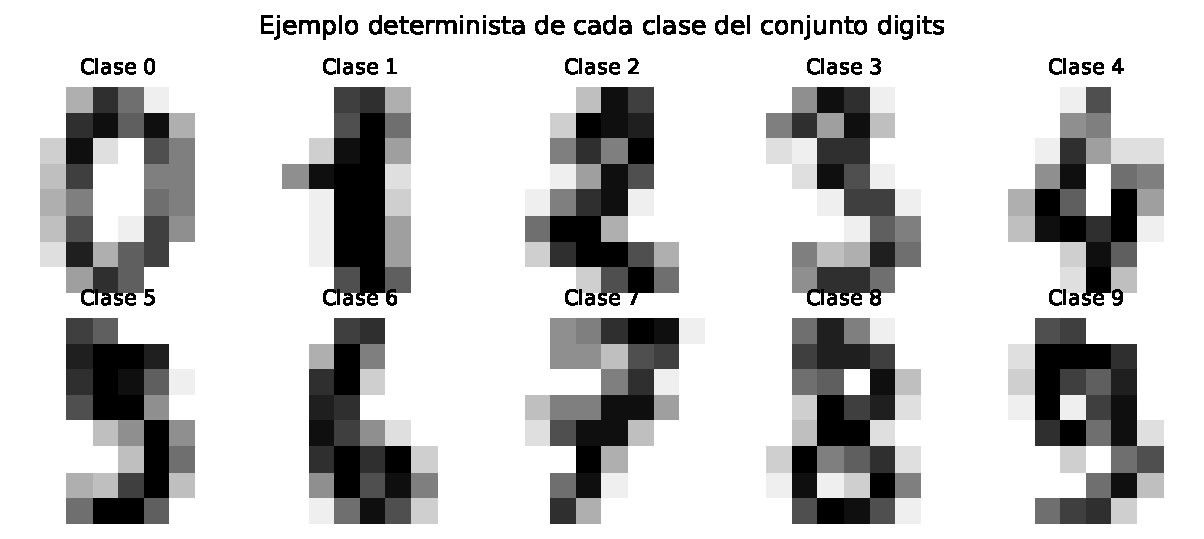
\includegraphics[width=0.82\textwidth]{dataset_examples}
  \caption{Una imagen seleccionada determinísticamente por cada clase. La resolución
  original es $8\times8$; la ampliación solo facilita la inspección visual.}
  \label{fig:dataset}
\end{figure}

Los índices se dividieron en \TrainSize{} observaciones de entrenamiento y
\TestSizeN{} de prueba (80/20), con estratificación por clase y semilla 42. El script
comprueba que no exista intersección entre ambas particiones.

\subsection{Modelo y evaluación predictiva}

Se ajustó un \texttt{RandomForestClassifier} \citep{breiman2001random} de
\NumTrees{} árboles, con selección de $\sqrt{64}$ atributos candidatos por división,
semilla 42 y los demás hiperparámetros predeterminados de scikit-learn. El bosque
recibe el vector aplanado de 64 intensidades. Se reportan exactitud, $F_1$ macro y
matriz de confusión. La probabilidad de una clase es el promedio de las probabilidades
estimadas por los árboles; dentro de cada árbol, esa estimación corresponde a la
fracción de muestras de la clase en la hoja alcanzada. No se aplicó calibración
adicional.

\section{Diseño de las explicaciones}

\subsection{TreeSHAP y referencia}

Para una imagen $x$ y una clase $c$, la explicación aditiva usada en este trabajo es
\begin{equation}
  f_c(x) = \phi_{0,c} + \sum_{j=1}^{64}\phi_{j,c},
  \label{eq:additivity}
\end{equation}
donde $f_c(x)$ es la probabilidad producida por el bosque, $\phi_{0,c}$ es el valor
esperado respecto a un conjunto de referencia y $\phi_{j,c}$ es la atribución del
píxel $j$. Se empleó \texttt{TreeExplainer} con perturbación
\emph{interventional} y salida en probabilidad. La referencia
contiene \BackgroundSize{} imágenes de entrenamiento: diez seleccionadas sin reemplazo
por cada clase con semilla 42. Por tanto, una atribución positiva significa que el
píxel eleva la salida respecto a \emph{esa referencia}; no significa que el píxel sea
causal ni universalmente importante.

Los mapas usan una escala divergente centrada en cero: rojo indica apoyo a la clase
mostrada y azul indica oposición. Se usa una escala común en los paneles para evitar
que la normalización independiente exagere diferencias pequeñas.

\subsection{Selección de tres imágenes}

Para evitar escoger manualmente ejemplos favorables, se fijaron tres reglas antes de
observar los mapas:
\begin{enumerate}
  \item el acierto cuya confianza está más cerca de la mediana de todos los aciertos;
  \item el acierto con el menor margen entre las dos clases más probables, excluyendo
  el caso anterior;
  \item el error de mayor confianza; si no hubiera errores, un segundo acierto de bajo
  margen.
\end{enumerate}
Todo empate se resuelve tomando el menor índice de la observación en el conjunto
original.
Para un acierto se contrasta la clase predicha con la segunda opción; para un error se
contrasta con la clase verdadera.

\subsection{Prueba de eliminación}

Una visualización coherente no garantiza fidelidad \citep{adebayo2018sanity}. Por ello
se ordenaron los píxeles según su SHAP para la clase predicha y se sustituyeron los
primeros $k\in\{1,2,4,8\}$ por la media del mismo píxel en la referencia. Los ocho
seleccionados tuvieron atribución positiva en todos los casos evaluados. Para cada
$k$, el control repite 200 selecciones uniformes entre los \RandomCandidateFeatures{}
píxeles con varianza no nula en la referencia; así se excluyen posiciones constantes
en ese fondo. Además, se calculó
\emph{drop@8} en todos los aciertos de prueba y se comparó cada caída SHAP con la media
de 100 máscaras aleatorias para esa misma imagen. Un bootstrap emparejado de $2\,000$
remuestreos resume la incertidumbre de la mediana de las diferencias. Esta intervención
se inspira en evaluaciones de eliminación, pero no reentrena el modelo
\citep{hooker2019benchmark}; solo prueba sensibilidad en entradas modificadas.

\section{Resultados}

\subsection{Desempeño del clasificador}

El modelo clasificó correctamente \CorrectTestCases{} de \TestSizeN{} imágenes y
cometió \IncorrectTestCases{} errores: exactitud \TestAccuracy{} y $F_1$ macro
\MacroFOne{}. La Figura~\ref{fig:confusion} permite localizar los pares de clases en
los que ocurrieron las confusiones, en lugar de reducir el desempeño a una sola cifra.

\begin{figure}[H]
  \centering
  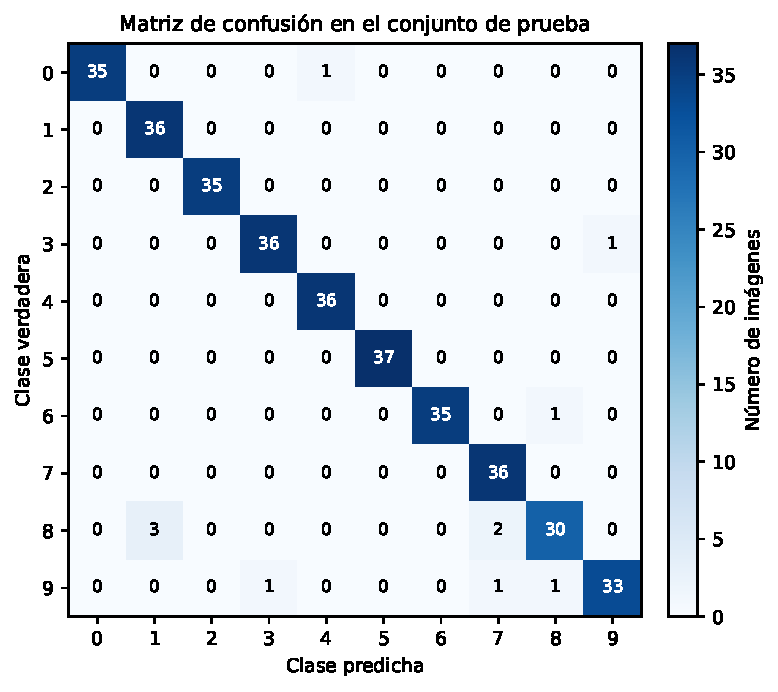
\includegraphics[width=0.60\textwidth]{confusion_matrix}
  \caption{Matriz de confusión de la partición de prueba. Los valores son conteos.}
  \label{fig:confusion}
\end{figure}

\subsection{Casos locales}

La Tabla~\ref{tab:cases} registra la selección exacta. El margen es la diferencia
entre las dos probabilidades más altas. Conservar el índice del conjunto completo
permite recuperar cada imagen sin archivos externos.

\begin{table}[H]
\centering
\small
\caption{Tres casos seleccionados por reglas deterministas.}
\label{tab:cases}
\begin{tabular}{c p{4.3cm} r c c r r c}
\toprule
Caso & Criterio & Índice & $y$ & $\hat y$ & $p(\hat y)$ & Margen & Acierto \\
\midrule
1 & Acierto de confianza mediana & 1089 & 3 & 3 & 0.817 & 0.727 & Sí \\
2 & Acierto correcto de menor margen & 1593 & 2 & 2 & 0.330 & 0.007 & Sí \\
3 & Error de mayor confianza & 1553 & 8 & 1 & 0.570 & 0.410 & No \\
\bottomrule

\end{tabular}
\end{table}

En la Figura~\ref{fig:shap}, la primera columna muestra la entrada, la segunda explica
la clase predicha y la tercera presenta una explicación contrastiva. Los mapas no
deben leerse como segmentaciones del trazo: cada celda expresa cuánto cambia la salida
del bosque en la descomposición de la Ecuación~\ref{eq:additivity}. La reconstrucción
de todas las salidas explicadas, incluidos los \CorrectTestCases{} aciertos usados en
la evaluación global, tuvo un error absoluto máximo de
\MaxAdditivityError, por debajo de la tolerancia predefinida de $10^{-5}$.

\begin{figure}[H]
  \centering
  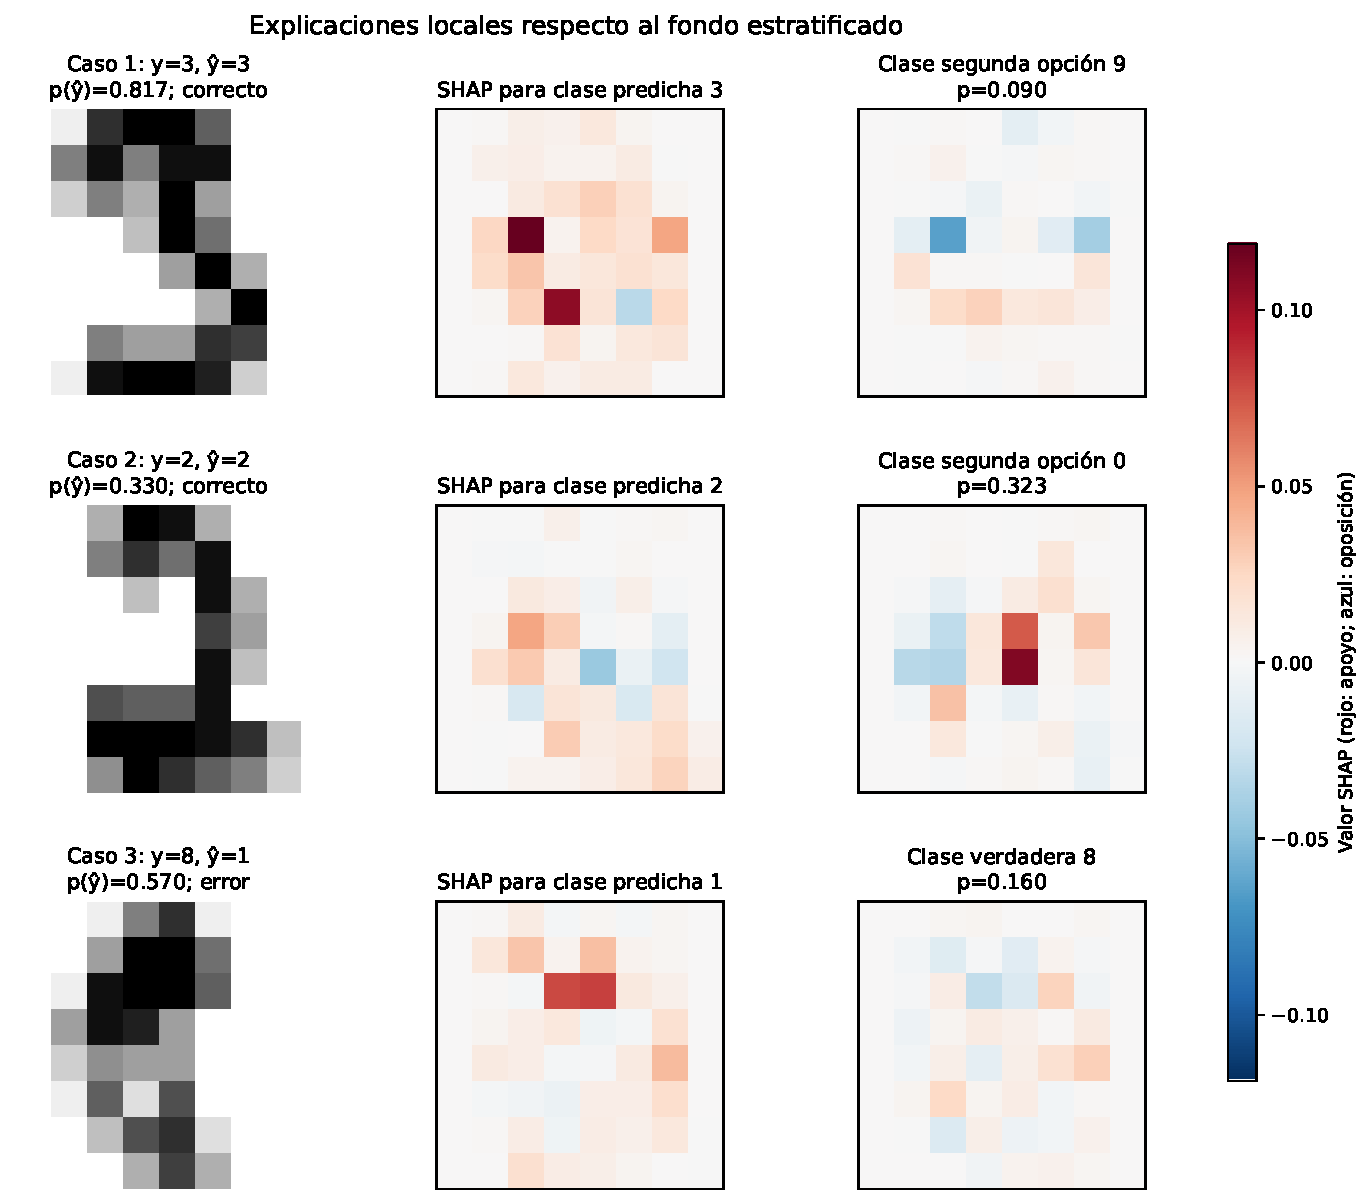
\includegraphics[width=\textwidth]{shap_explanations}
  \caption{Imágenes y mapas TreeSHAP. Rojo: aporte positivo; azul: aporte negativo,
  siempre respecto a la referencia estratificada. Para los aciertos se muestra como
  contraste la segunda clase más probable; para el error, la clase verdadera.}
  \label{fig:shap}
\end{figure}

\subsection{Sensibilidad por eliminación}

La Tabla~\ref{tab:deletion} presenta el resultado al sustituir ocho píxeles en cada
caso. Una caída positiva indica que la intervención redujo la probabilidad original.
Las curvas completas de la Figura~\ref{fig:deletion-selected} conservan también todos los
valores de $k$ y el intervalo percentil del control aleatorio.

\begin{table}[H]
\centering
\small
\caption{Eliminación de ocho píxeles en los casos seleccionados.}
\label{tab:deletion}
\begin{tabular}{crrrrr}
\toprule
Caso & $p_0$ & $p_{\mathrm{SHAP}}$ & Caída SHAP & $\bar p_{\mathrm{azar}}$ & Caída azar \\
\midrule
1 & 0.817 & 0.123 & 0.693 & 0.685 & 0.131 \\
2 & 0.330 & 0.100 & 0.230 & 0.304 & 0.026 \\
3 & 0.570 & 0.073 & 0.497 & 0.422 & 0.148 \\
\bottomrule

\end{tabular}
\end{table}

\begin{figure}[H]
  \centering
  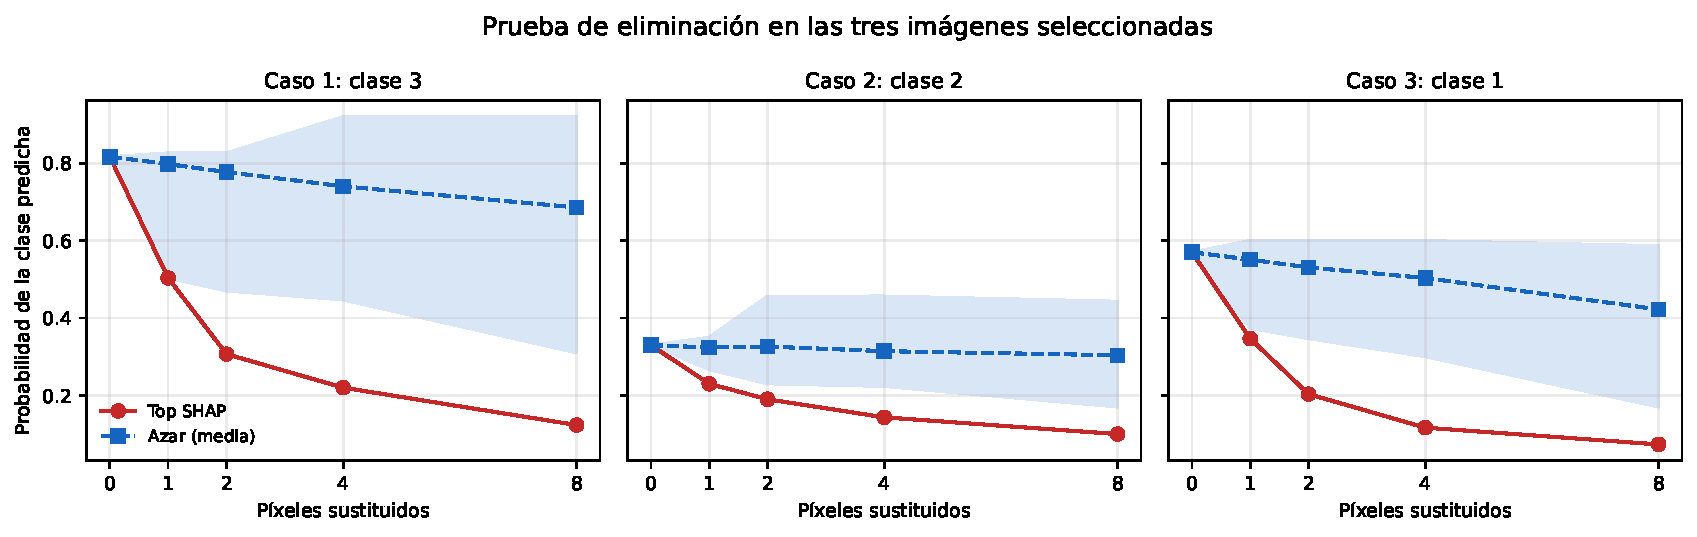
\includegraphics[width=\textwidth]{deletion_selected}
  \caption{Probabilidad de la clase originalmente predicha al sustituir píxeles. La
  banda azul es el intervalo percentil 2.5--97.5\% de 200 máscaras aleatorias.}
  \label{fig:deletion-selected}
\end{figure}

En el análisis global, la caída mediana fue \MedianShapDrop{} al sustituir los ocho
píxeles de mayor SHAP y \MedianRandomDrop{} para la media aleatoria. La diferencia
emparejada mediana fue \MedianPairedDifference{}, con intervalo bootstrap descriptivo
del 95\% [\DeletionCILow{}, \DeletionCIHigh{}]. La caída SHAP superó la caída aleatoria
media en \DeletionWinRate{} de los aciertos. Estos números evalúan la hipótesis de
sensibilidad planteada, no la corrección semántica ni la causalidad de cada mapa.

\begin{figure}[H]
  \centering
  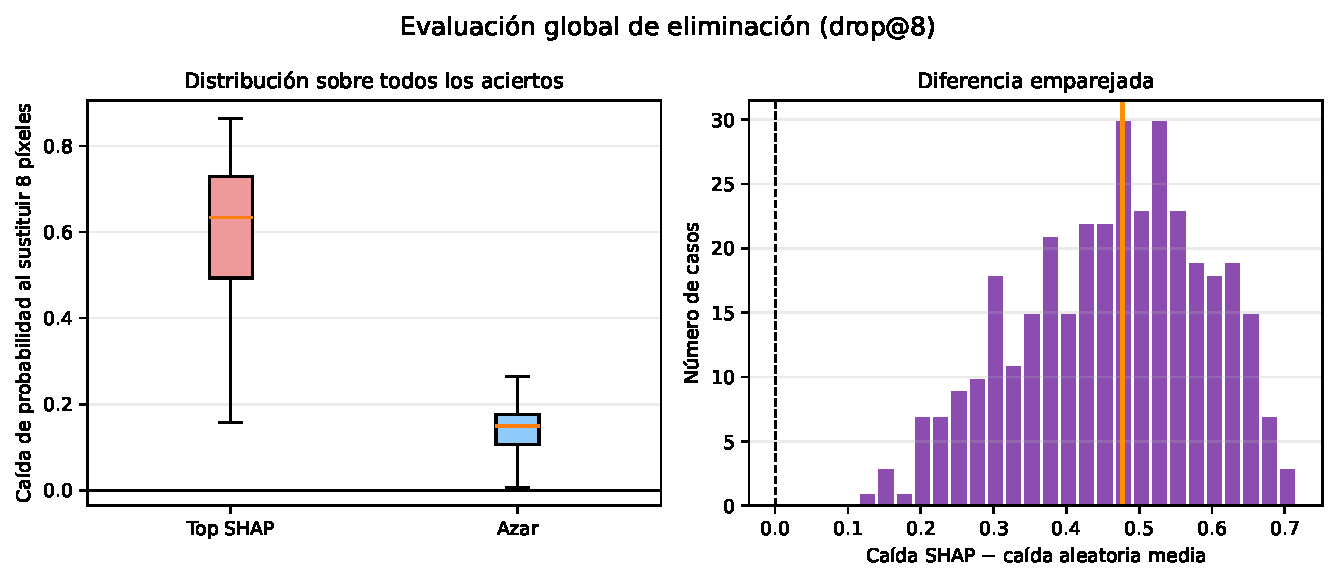
\includegraphics[width=0.91\textwidth]{deletion_global}
  \caption{Drop@8 sobre los \CorrectTestCases{} aciertos. Izquierda: distribuciones de
  caída, incluidos valores atípicos; derecha: diferencias emparejadas entre SHAP y el
  control aleatorio, con la mediana en naranja.}
  \label{fig:deletion-global}
\end{figure}

\section{Discusión y limitaciones}

El experimento relaciona tres niveles de evidencia: desempeño agregado, explicaciones
locales y una prueba de sensibilidad. La aditividad confirma que los valores reconstruyen
la salida explicada, mientras que la eliminación pregunta si los píxeles con atribución
alta afectan más la predicción que una selección sin información. Ninguna de las dos
comprobaciones demuestra que el modelo razone como una persona.

Las conclusiones están limitadas por los siguientes factores:
\begin{itemize}
  \item \textbf{Escala y dominio.} \texttt{digits} es pequeño, monocromático y de baja
  resolución; no representa el comportamiento de clasificadores sobre imágenes reales.
  \item \textbf{Arquitectura.} El bosque recibe 64 atributos planos y no modela
  explícitamente vecindad, traslación ni estructura espacial.
  \item \textbf{Referencia y dependencia.} Los valores SHAP cambian con la población de
  fondo y con el supuesto de perturbación. Los píxeles vecinos están correlacionados,
  de modo que repartir crédito entre ellos no tiene una única interpretación causal
  \citep{janzing2020feature}.
  \item \textbf{Entradas intervenidas.} Sustituir intensidades por medias puede crear
  imágenes fuera de la distribución. La prueba mide sensibilidad del modelo fijo y no
  incluye el reentrenamiento recomendado por protocolos como ROAR.
  Aunque se excluyen posiciones constantes, el control uniforme puede escoger píxeles
  de aporte pequeño o negativo; por ello, el
  porcentaje de victorias solo compara SHAP con este control concreto y no demuestra
  fidelidad general.
  \item \textbf{Alcance local.} Tres imágenes facilitan una auditoría concreta, pero no
  resumen toda la población. El análisis drop@8 amplía la comprobación únicamente a
  los aciertos de esta partición. Tanto el modelo como el bootstrap están condicionados
  a una sola división, semilla, referencia y realización de máscaras; el intervalo no
  incluye incertidumbre de reentrenamiento ni de generalización a otra población.
  \item \textbf{Probabilidad.} Las probabilidades del bosque no fueron calibradas; la confianza
  se interpreta como salida del modelo, no como frecuencia garantizada de acierto.
\end{itemize}

\section{Reproducibilidad}

El paquete incluye el código canónico, un notebook de ejecución, resultados tabulares,
figuras en PNG/PDF, el modelo serializado, bibliografía, registro de prompts y una lista
ampliada de limitaciones. La ejecución verificada utilizó Python \PythonVersion{},
scikit-learn \SklearnVersion{} y SHAP \ShapVersion{}. Desde la raíz, el flujo completo
en PowerShell es:
\begin{verbatim}
powershell -ExecutionPolicy Bypass -File .\reproduce.ps1
\end{verbatim}
El script crea un entorno Python 3.11 local, instala las dependencias directas con
versiones verificadas, ejecuta el
experimento, compila este documento y valida archivos, métricas, forma de las
atribuciones, aditividad y referencias LaTeX. Los valores numéricos se insertan desde
\texttt{results/generated\_values.tex}; las tablas también se generan automáticamente.

\section{Conclusiones}

TreeSHAP permitió descomponer, por clase y por píxel, tres predicciones de un bosque
aleatorio entrenado sobre dígitos manuscritos. Las reglas de selección explícitas, la
comprobación de aditividad y el control aleatorio de eliminación reducen decisiones
analíticas ocultas y hacen que las afirmaciones sean auditables. El ejercicio también
muestra el límite central de una explicación local: atribuir la salida de un modelo no
equivale a descubrir causas ni a validar el razonamiento humano. Para trabajos futuros,
convendría repetir el protocolo con imágenes de mayor resolución, modelos convolucionales,
varias referencias SHAP y pruebas que mantengan las intervenciones dentro de la
distribución de datos.

\section*{Declaración de asistencia y trazabilidad}

Se utilizó un asistente de IA para proponer la estructura, generar una primera versión
del código y del texto, y apoyar la verificación técnica. Las decisiones, comandos y
limitaciones están documentados en \texttt{prompts/prompt\_log.md} y
\texttt{LIMITATIONS.md}. Antes de entregar, la persona autora debe revisar las
afirmaciones, ejecutar el paquete y reemplazar el campo de autoría; la responsabilidad
final sobre el contenido no se delega al asistente.

\bibliographystyle{unsrtnat}
\bibliography{references}

\end{document}
